\documentclass[12pt]{article}

\usepackage{setspace}
\usepackage{graphicx}
\graphicspath{{./figs/}}

%% paragraph indent
\setlength\parindent{0pt}
%% 1.5 spacing
\setstretch{1.5}

%%
\renewcommand\thetable{\arabic{table}}
\renewcommand\thefigure{\arabic{figure}}

%%%%%%%% 
\begin{document}

\begin{titlepage}
\center 
\textsc{\LARGE Imperial College Business School}\\[1.0cm]
\textsc{\Large M.Sc., Business Analytics}\\[0.5cm]
\large Independent Study \\[1.5cm] 
{\bfseries Sentiment Analysis of Contact lens to predict sales and improve manufacturing process and quality }\\
{\large \today }\\[2cm] 
{\large \textbf \\ Author: Bharath Mukundakrishnan}
{\large \textbf \\ Prepared for\\ MiComp Soultions Inc. \\\tiny \textit{(An Agile Health Company)}\\\large Agile Health Technologies Inc.\\2728 Forgue Drive, Suite 106 Naperville, IL-60564} 
\end{titlepage}

\section*{Abstract}
In this study we undertake sentiment analysis to study feedback of customers that use contact lenses manufactured by Johnson\&Johnson Inc. Contact lenses, as an alternative to normal glasses, are used widely and offers many advantages. It is discreet, not subject to misplacement and offer aesthetic advantages that cannot be matched by normal glasses. However, since the lenses are worn on top of the iris, the quality of glass, the material of glass is quite important for customers to feel comfortable. Thus it is important for manufacturers of contact lenses to understand the sentiment(s) of people wearing these lens. Given the popularity of contact lenses over normal glasses, it is no surprise that there are various companies manufacturing them. There are also various brands of lenses manufactured by the same company in many cases. This study aims to study customer sentiments collected over a period of 10 years, sentiments pertaining to various brands of lenses. The result of the study will be used to see if there are trends and patterns in the uusage of these lenses. More importantly, it will allow the manufacturers of lenses to understand their own manufacturing process based on the sentiments expressed by the customers. We plan to use various machine learning methods to study the customer data and associate sentiments with rating for the product. We will develop a visualization dashboard that will allow managers to analyze slices of data over various vectors including date ranges, keywords and so on. A snapshot of raw data (XLS format) is shown in Figure \ref{fig:raw_data}.

\begin{figure}
  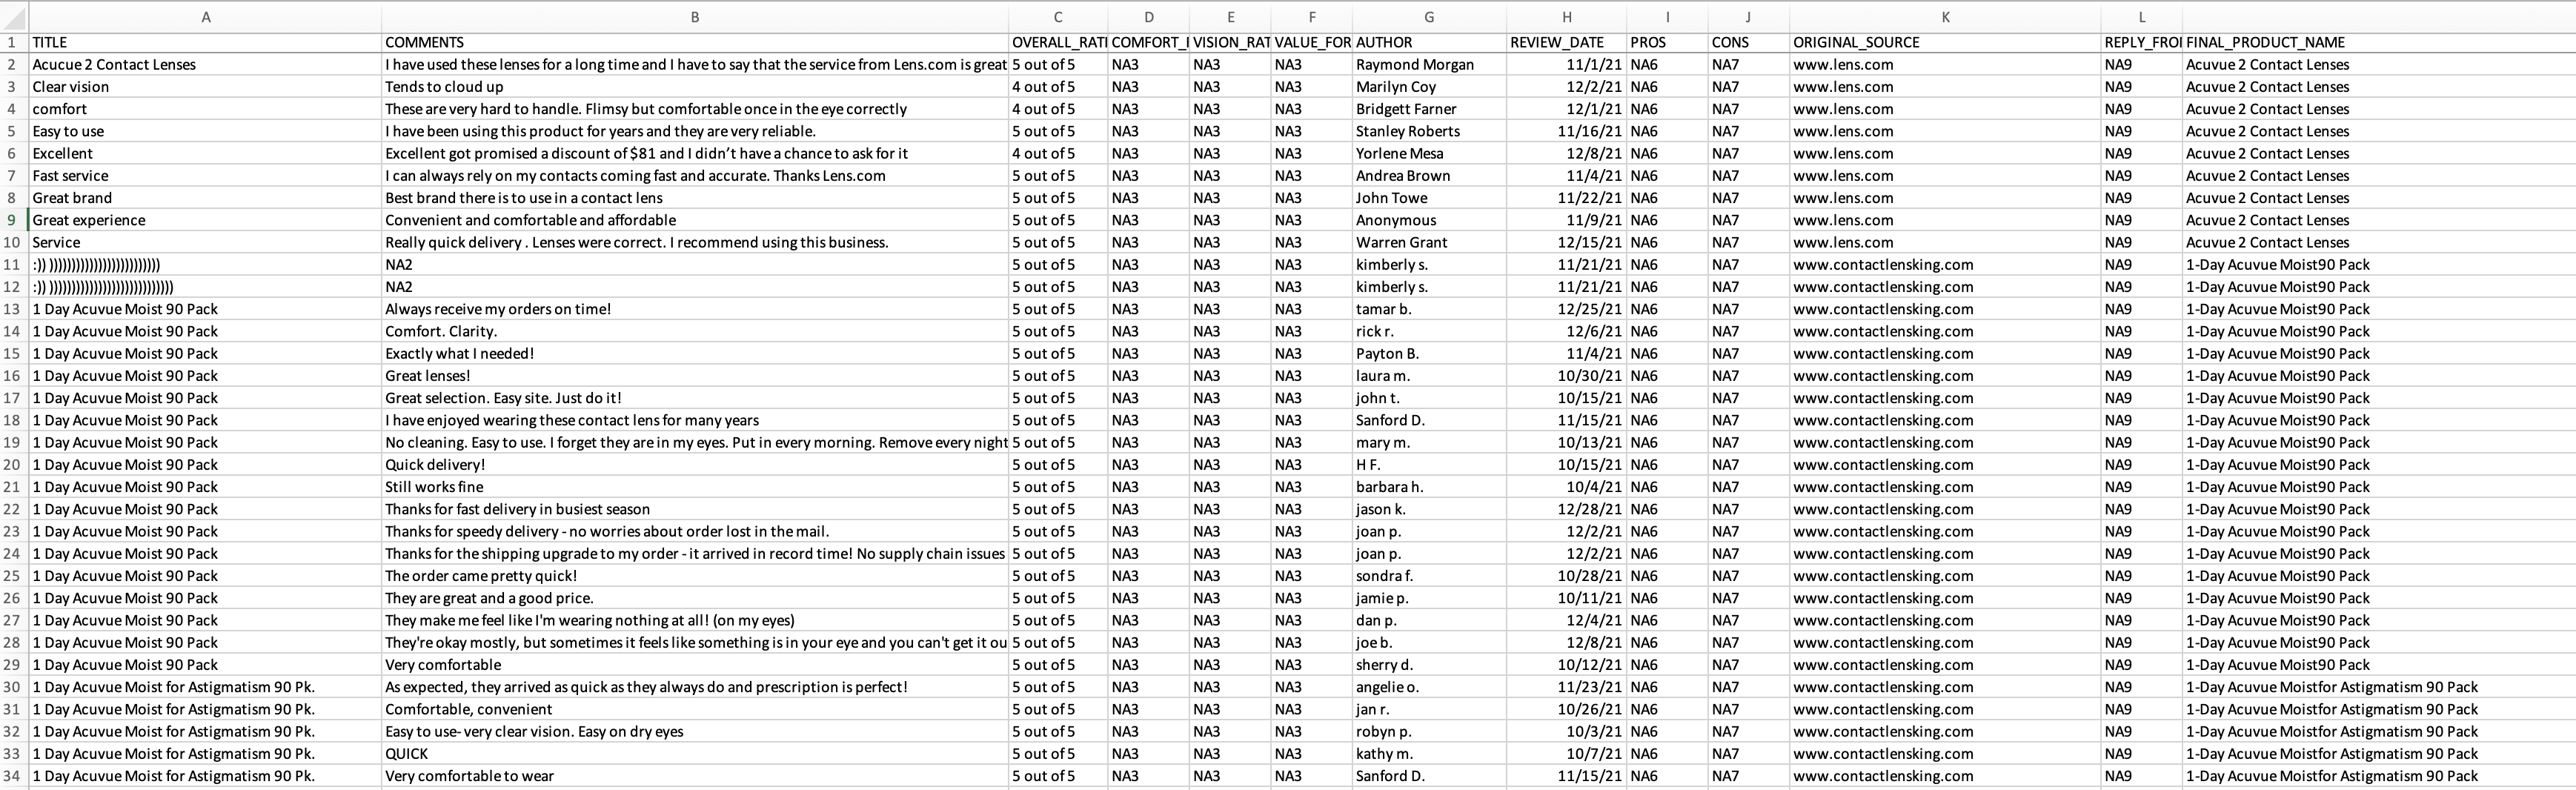
\includegraphics[width=\linewidth]{raw_data.png}
  \caption{Raw data}
  \label{fig:raw_data}
\end{figure}


\end{document}
%%%%%%%%
